\graphicspath{{fig/introduction/}}

\chapter{Introduction}
\label{cha:introduction}

\section{Motivation}
\label{sec:motivation}

Many of us have been struck by the inherent beauty of animals moving collectively; starlings gathering 
at dusk in huge numbers to perform the most mesmerising of ballets, the entire flock moving as if some 
fluid object; fish forming tight milling structures in defence against predation, changing direction in
 the blink of an eye and with a flash of silver. Collective motion has been observed over many differen
t length scales, and is not constrained only to vertebrates. At the mesoscale, studies have been made o
f turbulent microbial suspensions \parencite{dunkel13}. Swarms of locusts, which are capable of occupyi
ng up to one fifth of the Earth's land surface during a plague, are also known to exhibit collective mo
tion \parencite{bazazi08}.

\begin{figure}[!htbp]
	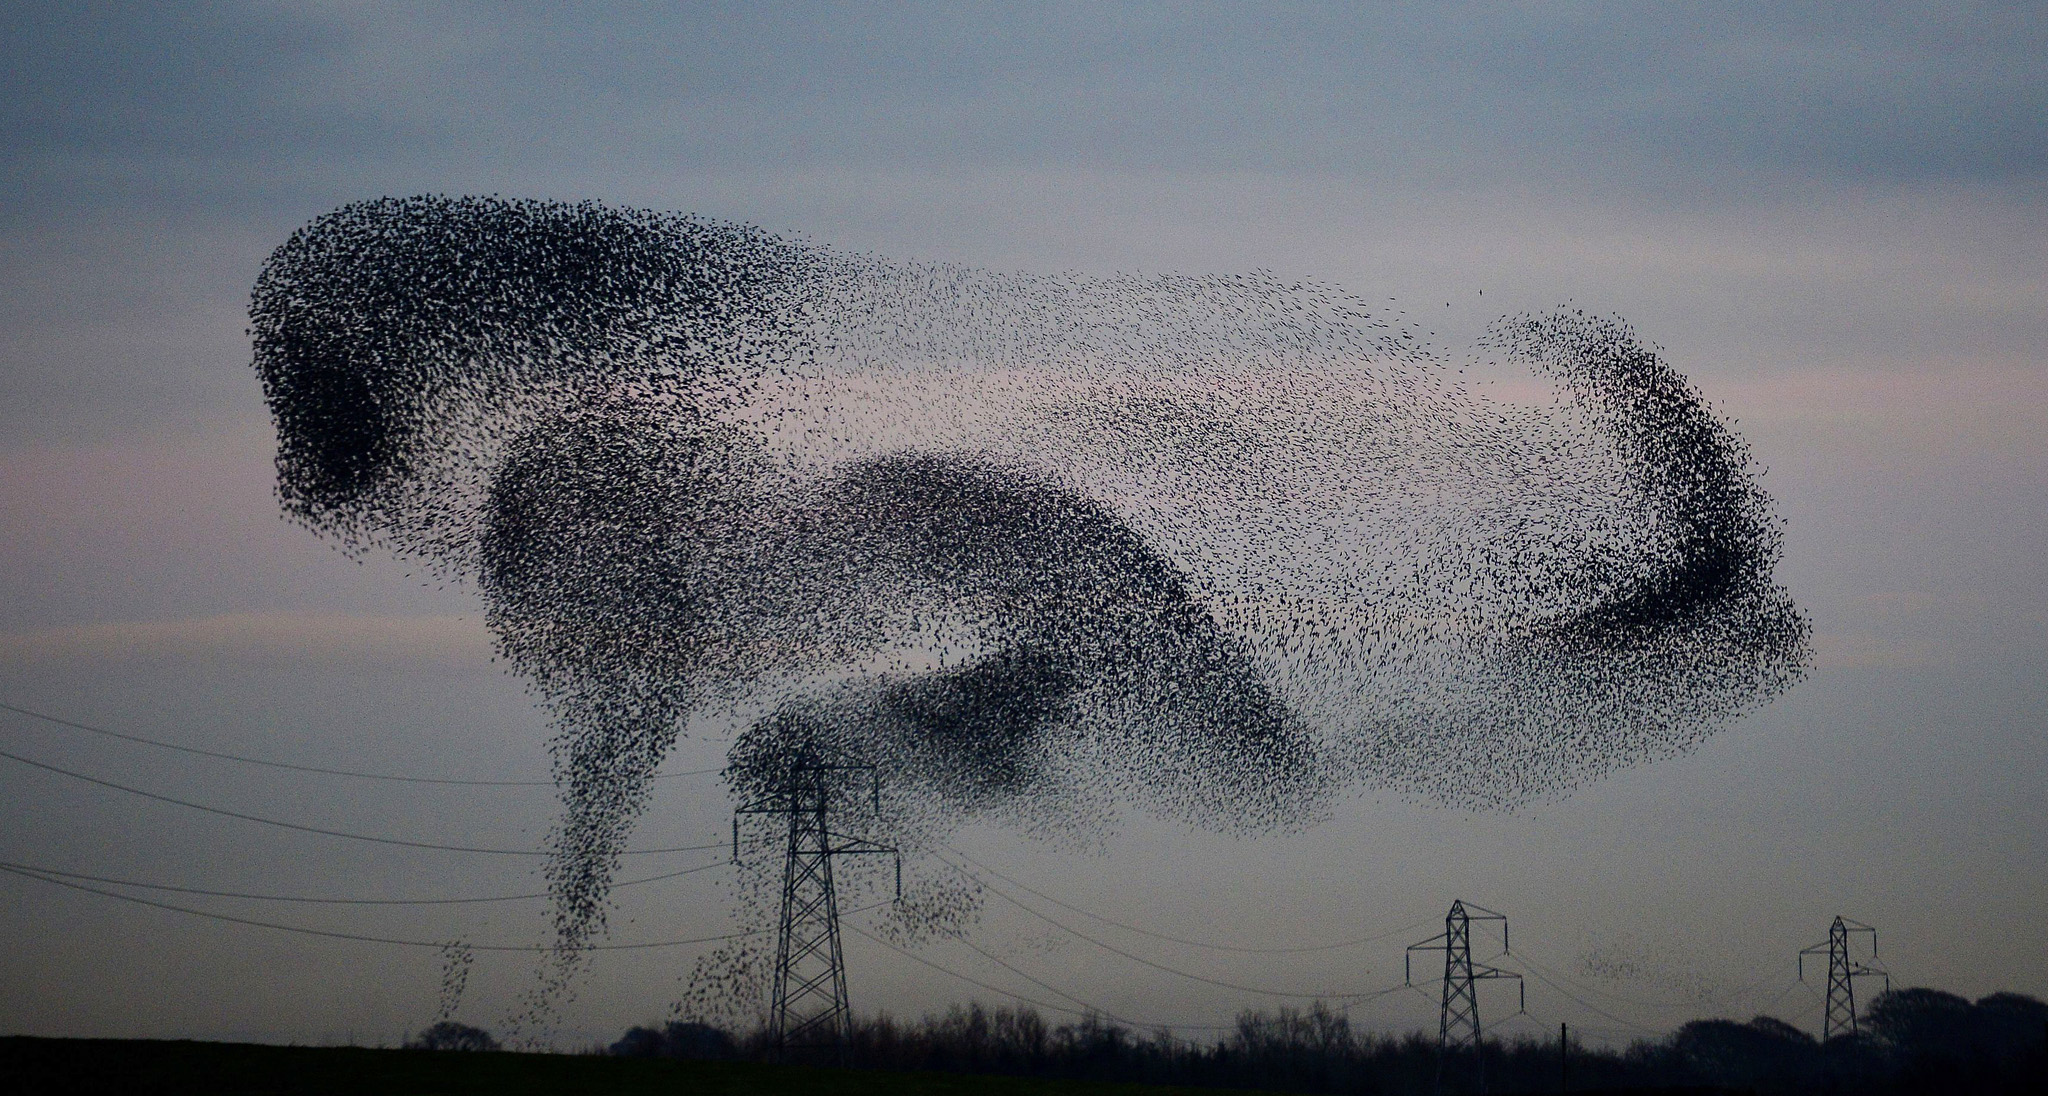
\includegraphics[width=\textwidth]{murmuration.jpg}
	\caption{A particularly startling example of a starling murmuration, captured near Gretna in the Scott
ish Borders. Photograph: Owen Humphreys/PA.}
	\label{fig:murmuration}
\end{figure}

Over the years collective behaviour has become a thriving topic of multidisciplinary research, capturin
g the imaginations of physicists, biologists, mathematicians and statisticians. Our understanding has e
volved significantly from early suggestions that collective behaviour results from thought-transference
 and telepathy between individuals \parencite{selous31}. Though we can often explain why animal aggrega
tions are evolutionary advantageous \parencite{giardina08}, much less is known about how these structur
es are formed and maintained.

Much work has been invested in developing theoretical models which seek to explain emergent behaviour b
y interactions at an individual level. Such models have shown that individual interactions are sufficie
nt to produce group-level structures. Many different simulations, implementing disparate interaction ru
les, are able to produce behaviour reminiscent of real flocking systems. However, these models have lar
gely only been verified with comparison to empirical observation at a qualitative level, and a thorough
 quantitative comparison between field data and theory has been lacking.

In recent years technological and methodological advances have made it possible to capture the movement
s of large groups of animal aggregates \parencite{ballerini08}. With this data, it is only now that we 
are in a position to make a robust comparison between model predictions and real-world observations.

\section{Overview of thesis}
\label{sec:overview_of_thesis}

We begin this thesis by giving the reader a review of the literature surrounding collective behaviour. 
Important results and ideas of the field are introduced and discussed. After relaying the main results 
from the literature we discuss open problems and the future of research in the field.

\cref{cha:bayes_intro} introduces the reader to the field of Bayesian statistics. Important results, te
chniques and algorithms from the field will be outlined as well as problems that the practitioner may e
ncounter, and how they may address these problems.

Now with a grasp of Bayesian statistics, the reader is given a short introduction to directional statis
tics in \cref{cha:direct_stats}. In this chapter we discuss why standard methods and techniques are ina
ppropriate for handling circular data. With the shortfalls of standard techniques considered, we introd
uce methods from the study of circular statistics which are appropriate to use with directional data.
